% Compile with pdfLaTeX using the official IEEEtran class.
\documentclass[conference]{IEEEtran}
\IEEEoverridecommandlockouts

\usepackage{cite}
\usepackage{amsmath,amssymb}
\usepackage{booktabs}
\usepackage{array}
\usepackage{graphicx}
\usepackage{xcolor}
\usepackage{url}
\usepackage{enumitem}
\usepackage{microtype}
\usepackage{pgfplots}
\pgfplotsset{compat=1.18}
% Plot coordinates below are derived from results/real CSV artifacts.
% Embedded vector figures keep this document self-contained.
\definecolor{coldblue}{RGB}{32,95,153}
\definecolor{coldorange}{RGB}{194,91,32}

% Standard IEEEtran conference layout; no margin or font-size overrides.
% Standalone source with IEEE conference formatting.
\title{ColdCast: Calibrated Cold-Start Prediction of AI System Performance\\
\large Project Checkpoint I}

\author{
\IEEEauthorblockN{Yi Chen Kuo, Sudip Manchare, Jaideep Manupati, Akshada Shailesh Rane}
\IEEEauthorblockA{Department of Computer Science, Virginia Tech, Alexandria, Virginia, USA\\
\{alvin9840, akshada, jaideepm21, msudip\}@vt.edu}
}

\begin{document}
\maketitle

\begin{abstract}
ColdCast predicts the probability that an AI system answers an unseen item correctly without executing that system. This checkpoint extends the proposal with a reproducible real-data pilot using 51,751 recorded responses and 1,345 normalized item-text groups from five measurement-db sources. Eleven predictors are evaluated with five source-held-out folds, a secondary item-held-out split, and three neural training seeds. Metadata logistic regression achieves item-held-out Brier score 0.1794, while the constant 0.5 predictor outperforms all learned models under source holdout (0.2500). Semantic fusion achieves 0.2738 and retrieval-enhanced fusion 0.2730 on that primary protocol. A separate limited-label experiment over 122 eligible system--source pairs reduces metadata-model Brier score from 0.2474 at zero labels to 0.1629 at 31 labels. These findings establish a working experimental pipeline, but do not establish a neural advantage or official competition performance. The report documents data selection, leakage controls, model configurations, limitations, individual responsibilities, and remaining deliverables.
\end{abstract}
\begin{IEEEkeywords}
Predictive AI evaluation, cold start, calibration, semantic representations, limited-label adaptation.
\end{IEEEkeywords}

\section{Introduction and Motivation}
Evaluating AI systems across many benchmark items can require substantial inference resources. Aggregate accuracy also conceals variation in item difficulty and system capabilities. Predictive evaluation instead estimates correctness probabilities from historical measurements, item content, and system metadata. The target is $\hat p_{s,i}=P(y_{s,i}=1\mid s,i)$, where $y_{s,i}$ is a recorded binary outcome. Such predictions are useful only if they generalize beyond the benchmarks supplying training labels.

ColdCast combines semantic item representations, system metadata, retrieval, and revealed labels. This checkpoint implements the proposal's frozen encoder, baselines, neural fusion, retrieval, calibration, and random-acquisition adaptation. All reported empirical results below use recorded measurement-db outcomes \cite{measurement}; earlier synthetic checks remain software tests and are excluded from the scientific result tables.

The central research question is: \textit{Can semantic fusion and limited-label adaptation improve calibrated correctness prediction for previously unseen benchmark sources?} We distinguish this from predicting new items within familiar sources. The distinction matters empirically: methods that perform well in the latter setting fail to outperform an uninformative probability of 0.5 in the former. 

The Stanford AIMS competition motivates the task \cite{aims}, but this study is an offline pilot rather than an official submission. Its zero-label source-held-out score and its local adaptation score use different populations and aggregation rules. Neither is presented as an official leaderboard result.

\section{Related Work and Study Contribution}
Amortized evaluation learns to predict measurements rather than repeatedly executing a target system. Truong et al. investigate reliable and efficient model-based evaluation \cite{truong2025}. Zhuang et al. connect AI evaluation with principles from human testing \cite{zhuang2023}. Item Response Theory (IRT) models system ability and item difficulty, providing a useful conceptual foundation, but its assumptions require scrutiny for AI evaluation \cite{jiang2026}. Contextual multidimensional IRT incorporates item information to address unseen questions \cite{shang2026}.

Our contribution is a reproducible ablation of metadata, lexical and semantic features, fusion, retrieval, and calibration under source holdout, followed by disjoint-pool label adaptation. We test three hypotheses: fusion improves zero-label Brier score; temperature scaling transfers across sources; and revealed labels reduce error. The first two are unsupported in this pilot; the third is supported descriptively.

\section{Dataset Construction and Audit}
\subsection{Versioned, Bounded Acquisition}
With approved access, we downloaded 37 metadata and tabular files (122.1 MB) from six collections, avoiding the full approximately 760-GB repository. The dataset revision is pinned to \texttt{54074453da7b}; the complete revision and per-file SHA-256 hashes are retained in the download manifest. Raw archives, execution traces, and image assets were not downloaded.

Five sources supply eligible binary responses: MathArena, Multi-SWE-bench, REAL web agents, ResearchCodeBench, and SWE-rebench. MMDocRAG was inspected and excluded because its fractional, multidimensional judge scores do not match binary correctness. MathArena additionally requires an explicitly binary grading scale: selecting only outcomes numerically equal to zero or one from a partial-credit rubric would produce an invalid binary subset. Items requiring unavailable image assets are excluded.

\begin{table}[t]
\caption{Selected real-data pilot. Groups denote distinct normalized item texts; systems denote evaluated configurations.}
\label{tab:data}\centering\small\setlength{\tabcolsep}{4pt}
\begin{tabular}{@{}lrrrr@{}}
\toprule
Source & Responses & Groups & Systems & Correct \\
\midrule
MathArena & 29,007 & 300 & 92 & 66.47\% \\
Multi-SWE-bench & 8,327 & 300 & 82 & 14.12\% \\
REAL web agents & 4,449 & 233 & 33 & 35.76\% \\
ResearchCodeBench & 6,784 & 212 & 31 & 36.13\% \\
SWE-rebench & 3,184 & 300 & 1 & 48.27\% \\
\midrule
Total & 51,751 & 1,345 & --- & --- \\
\bottomrule
\end{tabular}
\end{table}

\subsection{Sampling and Feature Eligibility}
Before model fitting, seed 5814 selects at most 300 normalized-text groups per source. Normalization lowercases text and collapses whitespace. All responses associated with a selected group are retained, including repeated trials and item identifiers that alias the same content. The resulting 1,412 item identifiers correspond to 1,345 text groups (Table~\ref{tab:data}). This preserves observed stochastic outcomes but means response-rich groups contribute more observations within a system's score.

Only pre-response item text and input metadata are eligible features. Reference answers, grading explanations, generated responses, and execution traces are excluded. System identity combines subject identity with run conditions rather than relying on a model's display name. Available metadata fields are normalized model name, provider, harness, reasoning effort, harness version, and system key. Missing values and unseen categories receive explicit fallback representations; approximately 37.3\% of selected MathArena responses lack provider metadata.

\subsection{Overlap and Coverage Checks}
Exact normalized text cannot cross evaluation partitions. Cross-source exact duplicates would be removed conservatively; none were found in this pilot. A frozen-embedding similarity audit found no cross-source pair with cosine similarity at least 0.98; the largest observed similarity was approximately 0.621. This is a diagnostic, not proof of independence: shared templates, paper families, related tasks, or paraphrases can escape these checks.

System coverage and success rates vary substantially (Table~\ref{tab:data}), making source shift central to interpretation. Raw data and model caches remain local; only code and aggregate results are intended for publication.

\section{Implemented Predictors}
\subsection{Statistical and Single-Modality Baselines}
The comparison includes constant 0.5, the global training correctness rate, and a smoothed per-system rate. For training successes $k_s$ and observations $n_s$, the latter is
\begin{equation}
\hat p_s=\frac{k_s+10\bar y_{\mathrm{train}}}{n_s+10}.
\end{equation}
An unseen system falls back to the global training rate. Metadata logistic regression uses training-fitted one-hot categories. TF--IDF logistic regression uses unigrams, a maximum vocabulary of 4,096, minimum document frequency two, and sublinear term frequency. Its vocabulary and inverse document frequencies are fitted on unique training items. Semantic logistic regression uses the frozen item embedding. All logistic models use $C=1$ and at most 500 solver iterations.

\subsection{Frozen Semantic Encoder and Fusion}
The item encoder is \texttt{all-MiniLM-L6-v2}, pinned to model revision \texttt{1110a243fdf4}; its complete identifier is saved with the run. Masked mean pooling followed by $L_2$ normalization produces 384-dimensional vectors. Inputs are limited to 256 tokens including special tokens. For longer inputs, the first 127 and last 127 content tokens are retained. This affects 602 of 1,345 groups; the median original length is 203 tokens and the longest is 54,192. Long coding and research tasks can therefore lose important context.

The fusion network concatenates the item vector with six learned eight-dimensional categorical embeddings. Hidden layers contain 64 and 32 ReLU units, with dropout 0.15 and a scalar output logit. Training randomly masks categories with probability 0.1 to exercise unknown-category behavior. The encoder remains frozen throughout; no target AI system is executed to generate new labels.


\subsection{Retrieval and Probability Calibration}
Retrieval uses the ten nearest training text groups by cosine similarity. Neighbor correctness rates are weighted by $\exp(\mathrm{similarity}/0.15)$, with a global training-rate prior of weight one. A training query excludes its own text group from its neighbors. This exclusion does not remove that group's contribution to the global training prior. Evaluation retrieval never uses development, calibration, or test outcomes. The resulting scalar is either a standalone prediction or an additional fusion input.

After fitting the network, temperature scaling transforms its logit $\ell$ into $\sigma(\ell/T)$. An independent calibration source selects among 81 log-spaced temperatures from 0.2 to 5 by response-weighted log loss. Both calibrated and uncalibrated variants are retained because calibration on one source need not transfer to another. Neural factorization, encoder fine-tuning, and active acquisition are not part of this implementation.

\section{Experimental Protocol and Reproducibility}
\subsection{Primary Source-Held-Out Evaluation}
Five folds hold out each source once. Sources are ordered as MathArena, Multi-SWE-bench, REAL web agents, ResearchCodeBench, and SWE-rebench. For each test source, the next source cyclically is development, the next is calibration, and the remaining two supply training data. Thus no source or normalized text group crosses roles within a fold. Training learns weights and category vocabularies; development selects the epoch; calibration selects temperature; test labels supply final evaluation only.

This protocol also introduces system cold starts. All test system configurations are unseen in training for four sources; for ResearchCodeBench, the unseen-configuration response fraction is approximately 56.2\%. Canonical model names can recur across configurations, so configuration holdout is not equivalent to holding out every model family. This distinction limits claims about generalization to entirely new foundation models.

\subsection{Secondary Item-Held-Out Diagnostic}
Within each source, normalized-text groups are divided approximately 60/15/10/15\% into training, development, calibration, and test. The resulting response counts are 31,703, 7,796, 5,009, and 7,243. Every test system and canonical model is represented in training. This measures new-item prediction with familiar systems. Different test populations and aggregation make the gap from source holdout descriptive, not a controlled estimate of shift cost.

\subsection{Training, Metrics, and Uncertainty}
Neural models use AdamW, learning rate 0.001, weight decay $10^{-4}$, batches of 1,024, and at most 40 epochs. Early stopping has patience seven and selects development macro Brier score. Seeds 5814, 5815, and 5816 vary neural initialization and training randomness; the data sampling and evaluation partitions remain fixed. Configurations are not retuned using test scores.

For a set of responses, Brier score is
\begin{equation}
B=\frac{1}{N}\sum_{j=1}^{N}(\hat p_j-y_j)^2.
\end{equation}
The primary metric first averages within each test system, then equally across systems in a source, then equally across five held-out sources. Neural results average these scores over three seeds. The item diagnostic averages equally across system--source pairs. Log loss and ten-bin, equal-width reliability diagnostics provide additional checks; pooled expected calibration error (ECE) is not a substitute for predictive performance.

Paired uncertainty intervals resample the five source clusters 5,000 times after averaging seeds. With only five clusters, these intervals are descriptive and unstable. Seed standard deviations capture optimization variation, not uncertainty from dataset selection, unseen benchmarks, or acquisition order.

\subsection{Executable Evidence}
The \texttt{checkpoint1/} pipeline saves data hashes, split audits, configurations, per-source metrics, predictions, checkpoints, and an environment lock. Seventeen automated tests pass across the original software fixture, real-data pipeline, and adaptation checks. All saved probabilities lie in the valid interval.

A separate offline inference check reloads a saved fusion checkpoint and independently encodes its input. It reproduces the stored prediction to an absolute difference of approximately $3.9\times10^{-8}$. Execution used local CPU resources and historical labels; the official competition interface remains untested.

\section{Results and Interpretation}
\subsection{Zero-Label Prediction}
\begin{table}[t]
\caption{Real-data Brier scores (lower is better). Item holdout and source holdout use different test populations and weighting. Neural values average three seeds.}
\label{tab:results}\centering\small
\begin{tabular}{@{}lrr@{}}
\toprule
Predictor & Item holdout & Source holdout \\
\midrule
Constant 0.5 & 0.2500 & \textbf{0.2500} \\
Global rate & 0.2486 & 0.2850 \\
Smoothed system rate & 0.1799 & 0.2825 \\
Metadata logistic & \textbf{0.1794} & 0.2699 \\
TF--IDF logistic & 0.2110 & 0.2825 \\
Semantic logistic & 0.2018 & 0.3335 \\
Retrieval only & 0.1910 & 0.2822 \\
Fusion & 0.1900 & 0.2738 \\
Fusion + temperature & 0.1887 & 0.2819 \\
Fusion + retrieval & 0.1884 & 0.2730 \\
Fusion + retrieval + temp. & 0.1886 & 0.2778 \\
\bottomrule
\end{tabular}
\end{table}

Metadata logistic regression is strongest on the secondary item split, with Brier 0.1794. The smoothed system rate is nearly as good at 0.1799, indicating that known-system history supplies substantial predictive information. Neither fusion variant improves upon these simple baselines. Semantic logistic regression improves on constant 0.5 within sources, but transfers poorly across sources.

On the primary protocol, every learned predictor is worse than constant 0.5 (Fig.~\ref{fig:comparison}). Fusion obtains 0.2738, retrieval-enhanced fusion 0.2730, and metadata logistic regression 0.2699. The result does not support the proposed neural advantage. Differences in source success rates, limited training-source diversity, unknown system configurations, and text truncation are plausible contributors, but the current experiment does not isolate their causal effects.

Fusion's source-held-out seed standard deviation is 0.0049; adding retrieval yields 0.0023. Relative to the smoothed system baseline, fusion's mean Brier difference is $-0.0087$, with a paired source-bootstrap interval approximately $[-0.0261,0.0062]$. Retrieval-enhanced fusion has difference $-0.0095$ and interval $[-0.0294,0.0080]$. Both include zero, so even superiority over that weaker baseline is not established.

\begin{figure}[t]
\centering
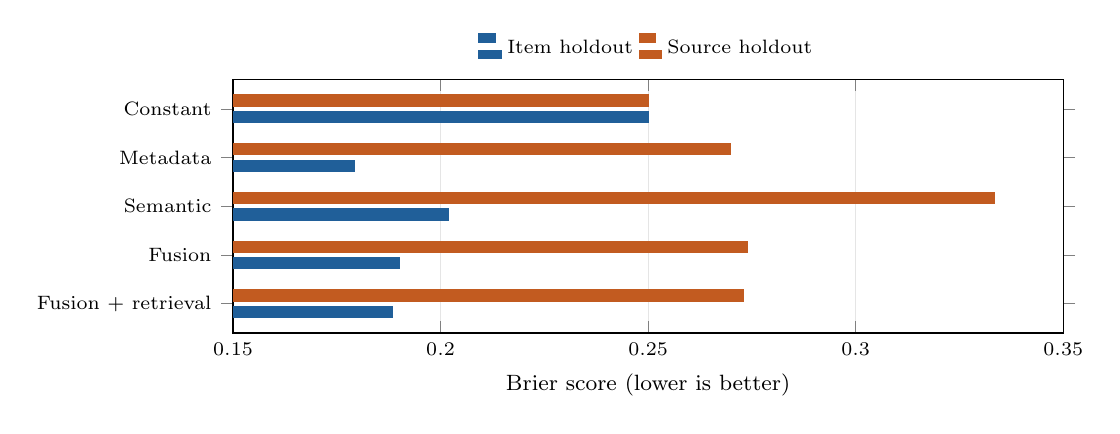
\begin{tikzpicture}
\begin{axis}[width=\columnwidth,height=4.8cm,scale only axis=false,
font=\footnotesize,xbar,bar width=4pt,xmin=0.15,xmax=0.35,
xtick={0.15,0.20,0.25,0.30,0.35},xlabel={Brier score (lower is better)},
ytick={1,2,3,4,5},yticklabels={Constant,Metadata,Semantic,Fusion,Fusion + retrieval},
y dir=reverse,ymin=0.4,ymax=5.6,xmajorgrids=true,grid style={gray!20},
legend style={at={(0.5,1.04)},anchor=south,legend columns=2,draw=none,font=\scriptsize},
tick label style={font=\scriptsize}]
\addplot[fill=coldblue,draw=coldblue] coordinates {(0.25000000,1) (0.17936978,2) (0.20178174,3) (0.18999052,4) (0.18835525,5)};
\addplot[fill=coldorange,draw=coldorange] coordinates {(0.25000000,1) (0.26987041,2) (0.33349827,3) (0.27383727,4) (0.27300413,5)};
\legend{Item holdout,Source holdout}
\end{axis}\end{tikzpicture}
\caption{Selected zero-label predictors. The horizontal scale starts at 0.15 to expose differences. Source holdout reverses the apparent benefit over constant 0.5. Protocols differ in population and weighting; Table~\ref{tab:results} reports all predictors.}
\label{fig:comparison}
\end{figure}

\subsection{Calibration Under Source Shift}
Temperature scaling improves fusion slightly on the item diagnostic (0.1900 to 0.1887), but worsens source-held-out Brier (0.2738 to 0.2819). Source-held-out fusion log loss is approximately 0.7524 and increases to 0.7759 after scaling; constant 0.5 gives 0.6931. Calibration labels from a different source therefore do not ensure better probability estimates on the test source.

Pooled ECE must also be interpreted carefully. The constant predictor has item-held-out ECE approximately 0.0017 because pooled correctness is close to one half, despite providing no item-level discrimination. Reliability plots are retained as diagnostics, while proper scoring rules and source-level breakdowns drive comparison.

\subsection{Limited-Label Adaptation}
A separate experiment includes 122 system--source pairs with at least 80 distinct text groups: 20 MathArena, 44 Multi-SWE-bench, 26 REAL, 31 ResearchCodeBench, and one SWE-rebench pair. Each pair receives a deterministic random 50/50 acquisition/evaluation split. Nested budgets $\{0,1,3,7,15,31\}$ reveal one sampled recorded response per selected acquisition group. Evaluation groups remain fixed and disjoint at every budget.

Given the base logit $\ell_i$, adaptation fits a scalar offset $\delta$ using acquired labels:
\begin{equation}
\min_{-5\leq\delta\leq5}\;\sum_{i\in A_b}\mathrm{BCE}\big(y_i,\sigma(\ell_i+\delta)\big)+\tfrac12\delta^2.
\end{equation}
At zero labels, $\delta=0$. The unit Gaussian prior regularizes small-budget updates. This correction changes the system--source success level without learning a new item representation.

\begin{table}[t]
\caption{Local adaptation on 122 eligible pairs. Brier at budgets 0 and 31 and weighted Brier ALC are pair-macro averages; lower is better. These are not official competition scores.}
\label{tab:adapt}\centering\small
\begin{tabular}{@{}lrrr@{}}
\toprule
Base predictor & 0 labels & 31 labels & ALC \\
\midrule
Metadata logistic & 0.2474 & \textbf{0.1629} & \textbf{0.1948} \\
Constant 0.5 & 0.2500 & 0.1634 & 0.1950 \\
Fusion + temperature & 0.2706 & 0.1635 & 0.2017 \\
Fusion + retrieval + temp. & 0.2707 & 0.1634 & 0.2017 \\
Fusion & 0.2908 & 0.1644 & 0.2082 \\
Smoothed system rate & 0.3062 & 0.1638 & 0.2124 \\
\bottomrule
\end{tabular}
\end{table}

Following the competition-inspired budget schedule \cite{aims}, local ALC weights budget scores by $(0.1,0.2,0.2,0.2,0.2,0.1)$. This experiment averages eligible system--source pairs equally, rather than weighting sources equally as in the primary zero-label table. Consequently, its zero-label values are not directly comparable to Table~\ref{tab:results}.

Adaptation lowers error for every evaluated base predictor (Table~\ref{tab:adapt}; Fig.~\ref{fig:adaptation}). Metadata logistic regression falls from 0.2474 to 0.1629, but adapting constant 0.5 nearly matches it. Their ALC difference is only about 0.00017 and is not evidence of a meaningful advantage. A simple label-based correction captures most of the observed benefit; a complex zero-label representation is not necessary for this pilot's adaptation gains. Only one acquisition trajectory is used per pair, fixed across neural seeds, so acquisition-order uncertainty remains unmeasured.

\begin{figure}[t]
\centering
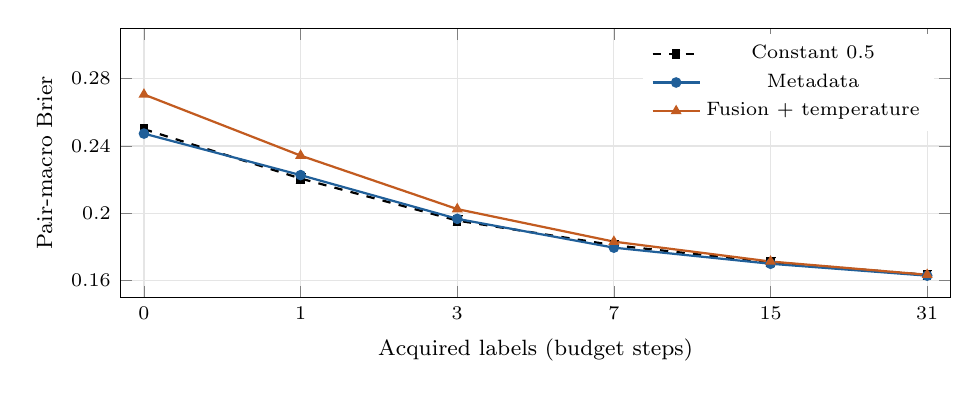
\begin{tikzpicture}
\begin{axis}[width=\columnwidth,height=5.0cm,font=\footnotesize,
xmin=-0.15,xmax=5.15,ymin=0.15,ymax=0.31,
xtick={0,1,2,3,4,5},xticklabels={0,1,3,7,15,31},
ytick={0.16,0.20,0.24,0.28},xlabel={Acquired labels (budget steps)},
ylabel={Pair-macro Brier},grid=major,grid style={gray!20},
legend style={at={(0.98,0.98)},anchor=north east,draw=none,font=\scriptsize},
tick label style={font=\scriptsize}]
\addplot[thick,mark size=1.5pt,black,dashed,mark=square*] coordinates {(0,0.25000000) (1,0.22065444) (2,0.19566859) (3,0.18099177) (4,0.17090573) (5,0.16341441)};
\addplot[thick,mark size=1.5pt,coldblue,mark=*] coordinates {(0,0.24736672) (1,0.22267935) (2,0.19669223) (3,0.17955812) (4,0.16999015) (5,0.16290769)};
\addplot[thick,mark size=1.5pt,coldorange,mark=triangle*] coordinates {(0,0.27059070) (1,0.23428377) (2,0.20248822) (3,0.18313861) (4,0.17132584) (5,0.16345679)};
\legend{Constant 0.5,Metadata,Fusion + temperature}
\end{axis}\end{tikzpicture}
\caption{Random-acquisition adaptation on 122 pairs with disjoint, fixed evaluation groups. Budget steps are equally spaced; values average three seeds with one shared acquisition trajectory per pair. Curves nearly converge at 31 labels. Acquisition-order uncertainty is not estimated.}
\label{fig:adaptation}
\end{figure}

\section{Project Progress and Team Responsibilities}
\label{sec:progress}
Completed project artifacts comprise the versioned data pilot, source- and item-held-out splits, eleven predictors, three-seed neural comparisons, retrieval and calibration ablations, limited-label adaptation, automated tests, and result visualizations. The following allocation defines four complementary areas of team responsibility; it does not assert equal amounts of completed individual work.

\textbf{Yi Chen Kuo---data preparation and validation.} Responsibilities cover binary-outcome eligibility, schema normalization, metadata quality, and sample coverage. The corresponding review artifacts are the dataset manifest, source-level data audit, and partition checks. This role also covers documenting duplicate-text controls and limitations of the selected pilot.

\textbf{Jaideep Manupati---predictive modeling and experiments.} Jaideep obtained dataset access and coordinated the checkpoint implementation and experiments. His modeling responsibilities cover statistical baselines, semantic representations, fusion architectures, training configurations, and interpretation of the source-held-out and item-held-out comparisons.

\textbf{Akshada Shailesh Rane---retrieval, calibration, and adaptation.} Responsibilities cover training-only retrieval, temperature scaling, acquisition/evaluation separation, and limited-label learning curves. The corresponding review artifacts are the retrieval ablations, calibration diagnostics, adaptation protocol, and budget-dependent results.

\textbf{Sudip Manchare---integration, reproducibility, and reporting.} Responsibilities cover pipeline integration, environment and configuration records, automated-test review, and saved-model inference verification. This role also covers consistency between result tables and figures, IEEE report integration, and maintenance of the project webpage.

Individual completion of the assigned reviews by Yi Chen, Akshada, and Sudip has not yet been documented. All members share responsibility for understanding the methodology, checking the reported evidence, and reviewing the final submission.

\section{Remaining Work and Limitations}
\subsection{Next Research Milestones}
The next research stage will expand source coverage and repeat acquisition trajectories before adding complexity. Planned ablations examine longer-context text representations, metadata missingness, and system-family separation. Calibration methods must be evaluated on genuinely shifted sources, with selection confined to development/calibration data. Active uncertainty and diversity acquisition will be compared against the implemented random policy using identical evaluation pools and budgets.

Future integration includes official inference/labeling interfaces, dependency packaging, resource limits, and end-to-end validation. Factorization and encoder fine-tuning are optional extensions.

\subsection{Threats to Validity}
Five source collections are too few to characterize general cold-start performance reliably. Sampling at most 300 text groups per source, preserving repeated outcomes, and having highly unequal system coverage affect the estimand. Exact-text grouping does not eliminate shared templates or hidden source overlap. Truncation removes much of some long inputs, while missing metadata weakens system descriptions. The frozen encoder may encode pretraining knowledge about benchmark content; this pilot does not audit its pretraining corpus.

The adaptation experiment uses recorded outcomes, one acquisition ordering per pair, and a restricted eligibility threshold. It does not simulate every deployment condition or measure active-selection benefits. Neither seed variability nor five-cluster bootstrap intervals justify broad statistical claims. These limitations motivate additional data and repeated protocols before architectural conclusions.

\section{Conclusion}
ColdCast has progressed from a proposal and synthetic checks to an executed real-data evaluation. The checkpoint's strongest finding is that familiar-source performance does not guarantee benchmark cold-start performance: all learned zero-label models trail constant 0.5 under source holdout. Limited-label adaptation improves results substantially, but a simple constant base is nearly as effective as metadata prediction. The next phase should test broader coverage and robust adaptation before claiming an advantage from neural fusion. The reproducible artifacts and documented team responsibilities provide a foundation for the next research stage.

\begin{thebibliography}{00}
\bibitem{aims} Stanford AI Measurement Science, ``Predictive AI Evaluation Competition,'' 2026. [Online]. Available: \url{https://aims.stanford.edu/competition/}
\bibitem{truong2025} S. Truong et al., ``Reliable and Efficient Amortized Model-based Evaluation,'' in \textit{Proc. ICML}, 2025.
\bibitem{zhuang2023} Y. Zhuang et al., ``Position: AI Evaluation Should Learn from How We Test Humans,'' in \textit{Proc. ICML}, 2025, arXiv:2306.10512v4.
\bibitem{jiang2026} H. Jiang et al., ``Can We Trust Item Response Theory for AI Evaluation?,'' arXiv:2607.15190, 2026.
\bibitem{shang2026} E. Shang, W. Tang, and Y. He, ``LLM Evaluation on Unseen Questions: Contextual Multidimensional IRT Model,'' arXiv:2608.22295, 2026.
\bibitem{measurement} AIMS Foundations, ``measurement-db,'' dataset card, accessed Oct. 19, 2026. [Online]. Available: \url{https://huggingface.co/datasets/aims-foundations/measurement-db}
\end{thebibliography}

\end{document}
